\documentclass[11pt, draft]{article}
 
\usepackage[margin=1in]{geometry} 
\usepackage{amsmath,amsthm,amssymb,bm}
\usepackage{ dsfont }
\usepackage{ bbold }
\usepackage{enumerate}
\newcommand{\N}{\mathbb{N}}
\newcommand{\Z}{\mathbb{Z}}
\usepackage{setspace}
\usepackage{titlesec}
\usepackage{hyperref}
\usepackage{booktabs}
\usepackage{adjustbox}
\usepackage{graphicx}
\usepackage{float}
\usepackage{natbib}
\usepackage{threeparttable}
\usepackage{enumitem}


\setstretch{1.2}

\begin{document}
% Title page
\begin{titlepage}
    \centering
    \vspace*{2cm}
    
    \vspace{0.5cm}

    \Large{\textbf{Title of the Research Paper:}}\\
    Viral Voting: A study in the information diffusion effects of different social pressure treatments on voter turnout.
    
    \vspace{0.5cm}

    \Large{\textbf{Author Name:}}\\
    \Large{Damanveer Singh Dhaliwal}\\
    \Large{Student ID: 1012787147}

    \vspace{0.5cm}
    
    \Large{\textbf{DRAFT Project One}}
    
    \vfill
    
    \large{Department of Economics}\\
    \large{University of Toronto}
    
    \vspace{0.8cm}
    
    \large{\today}
    
\end{titlepage}

\section{Introduction}
The most important aspect of a democratic society is the ability of its citizens to vote and select their representatives in the government. However, voter turnout has been declining consistently across all developed countries (\cite{solijonov_voter_nodate}). In the 2024 US Presidential Election, the voter turnout was $63.9\%$ percent, which was $2.7\%$ percent lower than the previous election. Similar trends can be observed in Canada, the UK, and Europe.

In order to ensure that representation across government levels is fair and stable, it is very important to understand what influences voter turnout. In their 2006 field experiment, Gerber, Green, and Larimer tackled this question and tried to isolate how voter turnout might be influenced by social pressures such as civic duty, peer pressure, etc. (\cite{gerber_social_2008}). Their research question studied the direct effects that the social pressure had on a voter turnout of a household. In this paper, we are going to use the data from their field experiment and isolate how information diffuses through a social network, especially concerning different types of social pressure. We want to study the diffusion effect of these different types of social pressures and how far they extend. 

Understanding how social pressure shapes information diffusion reveals to us the dynamics that neither phenomenon produces alone. And these dynamics have now provided some key results across public health, election results, and the spread of both knowledge and misinformation across billions of people. Across disciplines, researchers have found that information simply just does not diffuse through a network like a disease. It creates new societal rules and reshapes the very networks through which it spreads. 

\cite{hong_covid-19_2023} showed how positive social pressure from the public authority led to lower skepticism about the COVID-19 vaccine and increased vaccination rates. However, the study missed the effect of the information transfer among the citizens on the country and how that led to a positive outcome. \cite{bond_61-million-person_2012} found results similar to \cite{gerber_social_2008} where people who received social pressure treatments with familiar faces were 0.39\% more likely to vote than people who received a treatment with a stranger's face. \cite{bond_61-million-person_2012} also found that the social contagion/diffusion effect resulted in an additional 280,000 voters compared to the direct effects of approximately 60,000 voters. This is similar to the research question we are trying to anser in this study. However, we are trying to isolate the diffusion effects of different types of social pressure treatments.

\cite{atienza-barthelemy_modeling_2025} created a model to study the diffusion of information through social media. They found that social media allows for rapid dissemination of information but the longevity and the reach of the content is severely limited due to the availability of an overwhelming amount of information on these platforms. Given our data is from a field experiment in 2006, we are unable to study similar metrics, however, this can easily be a future extension of this project.

In a similar project, \cite{vosoughi_spread_2018} studied the spread of true and false news stories on Twitter. They found that false news had deeper and more rapid information diffusion effects. They also discovered that the diffusion effects of false news were human led and not influenced by bots. This is an interesting result and is the motivation behind our research question. We want to isolate which types of social pressure diffuse more effectively to combat misinformation as well as to allow for positive social pressure to be more effective. 

\cite{haenschen_social_2016} studied the effect of pride and shame social pressure treatments on voter turnout and found a treatment effect of 15.8\% to 24.3\%. However, they did not find any signficant effect from indirect social pressure or diffusion. Their empirical strategy was to use a linear probability model with OLS estimation. We will be using a similar empirical strategy but we will extend the empirical work to include spatial autoregressive models and causal machine learning methods to better isolate the diffusion effects.

The rest of the paper is structured as follows. Section 2 describes the original experiment and the data. Section 3 describes the theoretical framework and the empirical strategy. Section 4 presents the results and section 5 concludes. We do include a future extensions section after the conclusion to discuss how this project can be extended further.

\section{Data and Summary Statistics}
The data used in this project is from a field experiment conducted by \cite{gerber_social_2008} prior to the August 2006 primary elections in the state of Michigan, United States. The August 2006 primary election was a statewide election with offices across the political spectrum being contested. The data was collected from 180,002 households and every individual residing at the same address was considered to be a part of the household. Individuals with missing records, and individuals living in apartment complexes were not included. Individuals living on streets with fewer than 10 neighbours were also excluded from the experiment.

Prior to the random assigment of the treatment, individuals who were more likely to vote by an absentee ballot were excluded to control for pre-treatment voting decisions.Individuals who had not voted in the extremely high turnout 2004 general election were considered to have moved, died or double registered and were also excluded from the study.

The remaining 180,002 households were randomly assigned to one of the four treatment groups or the control group. The control group received no mailings. Each household in one of the treatment groups received one of the four mailings 11 days prior to the election. Each mailing included ``DO YOUR CIVIC DUTY - VOTE!" along with a varying degree of social pressure. The four treatment groups were as follows:

The \textbf{Civic Duty} treatment was the least intrusive and included the message: ``Remember your rights and responsibilities as a citizen. Remember to vote." The \textbf{Hawthorne} treatment told households ``YOU ARE BEING STUDIED" and that their voting behaviour was being monitored for research purposes. The \textbf{Self} treatment included a message that informed the household that their voting record was public information and included their public record for the previous elections. Finally, the \textbf{Neighbors} treatment was the most intrusive and included a message that informed the household that their voting record was public information and included their public record for the previous elections. Additionally, it also included the voting records of their neighbours.
Both the Self and the Neighbors treatments included the face that an updated voting record would be mailed to them after the election.

The outcome variable of interest is whether an individual voted in the August 2006 primary election. The data also collected information from the previous elections in 2000, 2002 and 2004 that was supplemented from the Qualified Voter File. Finally, the data included demographic information such as age, gender and party affiliation couped with census data of the household's neighbourhood.

\begin{table}
\caption{Summary Statistics}
\label{tab:summary_stats}
\begin{tabular}{lrrrrrrrrrrrrr}
\toprule
 & sex & yob & g2000 & g2002 & g2004 & p2000 & p2002 & voted & treatment_control & treatment_self & treatment_civic duty & treatment_neighbors & treatment_hawthorne \\
\midrule
count & 344084.00 & 344084.00 & 344084.00 & 344084.00 & 344084.00 & 344084.00 & 344084.00 & 344084.00 & 344084.00 & 344084.00 & 344084.00 & 344084.00 & 344084.00 \\
mean & 0.50 & 1956.21 & 0.84 & 0.81 & 1.00 & 0.25 & 0.39 & 0.32 & 0.56 & 0.11 & 0.11 & 0.11 & 0.11 \\
std & 0.50 & 14.45 & 0.36 & 0.39 & 0.00 & 0.43 & 0.49 & 0.46 & 0.50 & 0.31 & 0.31 & 0.31 & 0.31 \\
min & 0.00 & 1900.00 & 0.00 & 0.00 & 1.00 & 0.00 & 0.00 & 0.00 & 0.00 & 0.00 & 0.00 & 0.00 & 0.00 \\
max & 1.00 & 1986.00 & 1.00 & 1.00 & 1.00 & 1.00 & 1.00 & 1.00 & 1.00 & 1.00 & 1.00 & 1.00 & 1.00 \\
count_0 & - & - & 54095.00 & 64942.00 & 0.00 & 257464.00 & 209947.00 & 235388.00 & 152841.00 & 305866.00 & 305866.00 & 305883.00 & 305880.00 \\
count_1 & - & - & 289989.00 & 279142.00 & 344084.00 & 86620.00 & 134137.00 & 108696.00 & 191243.00 & 38218.00 & 38218.00 & 38201.00 & 38204.00 \\
\bottomrule
\end{tabular}
\end{table}

Since the variables are binary, the summary statistics do not offer much insight. However, we can see that the treatment groups are fairly evenly distributed with the control group being slightly larger. The average age of the individuals in the sample is 50 years old. Below is a bar chart showing the outcome variable (voted in 2006 election) based on previous voting history.
\begin{figure}[H]
    \centering
    \includegraphics[width=1\textwidth]{../Output/Plots/figure1.png}   
    \caption{Voter Turnout in 2006 Election by Previous Voting History}
    \label{fig:figure1}
\end{figure}

As expected, individuals who voted in the previous elections were more likely to vote in the 2006 election. However, it is interesting to see that even after excluding everyone who did not vote in the 2004 general elections, there was a signficant portion of individuals who did not vote in the 2004 primary elections but voted in the 2006 primary elections. This shows that there are individuals who are not regular voters but can be mobilized to vote. 

The data was downloaded from a Stanford GSB \href{https://github.com/gsbDBI/ExperimentData}{repository}. Given the field experiment's thorough design and randomization, we are confident that the data is of high quality and can be used for our analysis. The data was already cleaned and there are no major issues with missing data or outliers.


\pagebreak

\section{Theoretical Model \& Empirical Framework}
To model the information diffusion effects of social pressure on voting, we will borrow a network diffusion model from \cite{myers_information_2012}. The original model is designed to capture the spread of information through a social network. In our case, we will adapt the model to capture it based on geographical proximity. Effects are bound to be different since social media connections allow for rapid and far reaching dissemination of information.

\subsection{Model Description}
The original model by \cite{myers_information_2012} has three main components: the contagion, internal exposure and external exposure. With respect to the reserach question at hand, we define these components as follows:

We define \textbf{contagion} as the information about social pressure and the public disclosure of voting behaviour. A household becomes 'infected' when they become aware that (1) voting behavior is being monitored, (2) their voting records may be publicized to neighbors, and (3) voting is subject to social surveillance. This information can spread through both the experimental mailings and through social diffusion within neighborhoods.

An \textbf{internal exposure} occurs when a household learns about the social pressure treatments from their neighbors who received the mailings. This includes both direct social interactions (neighbors discussing the mailings) and indirect observations (seeing neighbors vote, observing physical mailings, or experiencing increased social pressure within the neighborhood). Internal exposures capture all information transmission along the edges of our observed network structure.

\textbf{External exposures} represent the instances when information reaches a household from sources outside their immediate neighbor network. This includes the experimental mailings themselves (the primary observed external exposure), as well as unobserved sources such as local media coverage, family members living elsewhere, workplace discussions, and general get-out-the-vote campaigns occurring simultaneously. External exposures represent information 'jumping into' the network from outside.

\subsection{Model}
The original model in \cite{myers_information_2012} models the probability of infection at time t as:

\begin{equation*}
    F^{(i)}(t) = \sum_{n=1}^{\infty} P[i \text{ has } n \text{ exp. }] \times P[i \text{ inf. } | i \text{ has } n \text{ exp. }]
\end{equation*}
\begin{equation*}
    = \sum_{n=1}^{\infty} P_{\exp}^{(i)}(n; t) \times \left[ 1 - \prod_{k=1}^{n} [1 - \eta(k)] \right].
\end{equation*}

Where $P_{\exp}^{(i)}(n; t)$ is the probability that node $i$ has received $n$ exposures by time $t$ and $\eta(k)$ is the probability of infection upon the $k^{th}$ exposure.

Similarly, we model the probability that a household votes as a function of both internal and external exposures. However, \cite{myers_information_2012} developed a dynamic model that tracks how probability evolves over time as repeated exposures occur. This requires temporal data on when households decided to vote, which we do not have. Therefore, we borrow their framework and apply two simplifying approaches that captures the same mechanism in a static setting.

\subsubsection{Linear Model}
In order to simplify the model, we integrate over time and apply a linear approximation to get the following static model:
\begin{equation*}
    P(\text{vote}_i = 1) = \beta_0 + \beta_1 \cdot \text{treatment}_i + \beta_2 \cdot \text{neighbors\_treated}_i + \gamma X_i + \alpha_{\text{block}} + \varepsilon_i
\end{equation*}
where:
\begin{itemize}[noitemsep]
    \item $\text{treatment}_i$ is a binary indicator for whether household $i$ received a mailing (captures external exposure)
    \item $\text{neighbors\_treated}_i$ is the count of $i$'s neighbors who received mailings (captures internal exposure)
    \item $X_i$ is a vector of individual characteristics (age, sex, past voting history)
    \item $\alpha_{\text{block}}$ are block fixed effects (control for neighborhood-level confounders)
    \item $\varepsilon_i$ is the error term (clustered at household level, the unit of randomization)
\end{itemize}


The key parameters of interest are $\beta_1$ and $\beta_2$. $\beta_1$ captures the direct effect of receiving a social pressure mailing on the probability of voting (the external exposure), while $\beta_2$ captures the diffusion effect from having more neighbors treated (the internal exposure). A positive and significant $\beta_2$ would indicate that information about social pressure diffuses through neighborhood interactions, increasing voter turnout even among untreated households.

\subsubsection{Graphical Neural Network Model}
To capure potential non-linearities and complex interactions in the diffusion process, we will employ Graphical Neural Networks (GNNs) (\cite{kipf_semi-supervised_2017}). GNNs are well-suited to replicate the network structure of neighborhoods that \cite{myers_information_2012} originally modeled. In this approach, each household is represented as a node in a graph, with edges connecting neighboring households. The GNN will learn to predict the probability of voting based on both individual features and the features of neighboring nodes.

GNNs can also capture higher-order interactions that may be present in the diffusion of social pressure information. For example, the influence of a neighbor who has a treated neighbor. \cite{myers_information_2012} also has a non-linear exposure curve that can be better captured with a non-linear model like the GNN.

GNNs stack non-linear convolutional layers of the form:
\begin{equation*}
    H^{(l+1)} = \sigma(\tilde{D}^{-\frac{1}{2}}\tilde{A}\tilde{D}^{-\frac{1}{2}}H^{(l)}W^{(l)})
\end{equation*}
where $\tilde{A} = A + I$ is the adjacency matrix of an undirected graph with added self-connections. $I_N$ is the identity matrix, $\tilde{D}_{ii} = \sum_j \tilde{A}_{ij}$ and $W^{(l)}$ is a layer-specific trainable weight matrix. $\sigma(\cdot)$ is an activation function with the most popular choice being ReLU ($f(x) = \max(0,x)$). ReLU is computationally efficient and helps mitigate the vanishing gradient problem.

For our application, the input layer $H^{(0)}$ will consist of individual features such as the treatment assignmen, age, gender, and past voting history. Variable selection will be performed using regualarization techniques and random forest feature importance scores. The output layer $H^{(L)}$ will produce the predicted probability of voting for $L$ hops in the neighborhood graph.

\section{Regression Results \& Other Models}
\subsection{OLS}
To estimate the direct effects of the different social pressure treatments on voter turnout, we will explore all the widely used econometric methods in the literature. We will start with a simple OLS regression of the form:
\begin{equation}
    Y_i = \beta_0 + \beta_1 CivicDuty_i + \beta_2 Hawthorne_i + \beta_3 Self_i + \beta_4 Neighbors_i + \epsilon_i
\end{equation}
Where $Y_i$ is a binary variable that takes the value of 1 if the individual voted in the 2006 primary election and 0 otherwise. $CivicDuty_i$, $Hawthorne_i$, $Self_i$ and $Neighbors_i$ are binary variables that take the value of 1 if the individual was assigned to that treatment group and 0 otherwise. The control group is the omitted category. $\epsilon_i$ is the error term.
Control variables for age, gender, and previous voting history will be added to the regression to increase precision. We will also cluster the standard errors at the household level to account for any correlation in the error terms within households.
\begin{equation}
    Y_i = \beta_0 + \beta_1 CivicDuty_i + \beta_2 Hawthorne_i + \beta_3 Self_i + \beta_4 Neighbors_i + \beta_5 X_i + \epsilon_i
\end{equation}
Where $X_i$ is a vector of control variables. Results from the regression are presented in Table 2. 
\begin{table}[H]
    \begin{center}
\begin{tabular}{lclc}
\toprule
\textbf{Dep. Variable:}        &      voted       & \textbf{  R-squared:         } &      0.054   \\
\textbf{Model:}                &       OLS        & \textbf{  Adj. R-squared:    } &      0.054   \\
\textbf{Method:}               &  Least Squares   & \textbf{  F-statistic:       } &      2245.   \\
\textbf{Date:}                 & Tue, 30 Sep 2025 & \textbf{  Prob (F-statistic):} &      0.00    \\
\textbf{Time:}                 &     11:26:19     & \textbf{  Log-Likelihood:    } & -2.1513e+05  \\
\textbf{No. Observations:}     &      344084      & \textbf{  AIC:               } &  4.303e+05   \\
\textbf{Df Residuals:}         &      344073      & \textbf{  BIC:               } &  4.304e+05   \\
\textbf{Df Model:}             &          10      & \textbf{                     } &              \\
\textbf{Covariance Type:}      &       HC1        & \textbf{                     } &              \\
\bottomrule
\end{tabular}
\begin{tabular}{lcccccc}
                               & \textbf{coef} & \textbf{std err} & \textbf{z} & \textbf{P$> |$z$|$} & \textbf{[0.025} & \textbf{0.975]}  \\
\midrule
\textbf{treatment\_civic duty} &       0.0181  &        0.003     &     7.176  &         0.000        &        0.013    &        0.023     \\
\textbf{treatment\_hawthorne}  &       0.0254  &        0.003     &    10.011  &         0.000        &        0.020    &        0.030     \\
\textbf{treatment\_neighbors}  &       0.0815  &        0.003     &    31.102  &         0.000        &        0.076    &        0.087     \\
\textbf{treatment\_self}       &       0.0482  &        0.003     &    18.701  &         0.000        &        0.043    &        0.053     \\
\textbf{sex}                   &      -0.0059  &        0.002     &    -3.817  &         0.000        &       -0.009    &       -0.003     \\
\textbf{yob}                   &      -0.0026  &     5.97e-05     &   -43.618  &         0.000        &       -0.003    &       -0.002     \\
\textbf{g2000}                 &      -0.0238  &        0.002     &   -10.203  &         0.000        &       -0.028    &       -0.019     \\
\textbf{g2002}                 &       0.0979  &        0.002     &    47.363  &         0.000        &        0.094    &        0.102     \\
\textbf{g2004}                 &       5.2626  &        0.118     &    44.654  &         0.000        &        5.032    &        5.494     \\
\textbf{p2000}                 &       0.0959  &        0.002     &    50.105  &         0.000        &        0.092    &        0.100     \\
\textbf{p2002}                 &       0.1149  &        0.002     &    67.454  &         0.000        &        0.112    &        0.118     \\
\bottomrule
\end{tabular}
\begin{tabular}{lclc}
\textbf{Omnibus:}       & 497112.529 & \textbf{  Durbin-Watson:     } &     1.906  \\
\textbf{Prob(Omnibus):} &    0.000   & \textbf{  Jarque-Bera (JB):  } & 51799.012  \\
\textbf{Skew:}          &    0.720   & \textbf{  Prob(JB):          } &      0.00  \\
\textbf{Kurtosis:}      &    1.759   & \textbf{  Cond. No.          } &  2.94e+05  \\
\bottomrule
\end{tabular}
%\caption{OLS Regression Results}
\end{center}

Notes: \newline
 [1] Standard Errors are heteroscedasticity robust (HC1) \newline
 [2] The condition number is large, 2.94e+05. This might indicate that there are \newline
 strong multicollinearity or other numerical problems.
    \caption{OLS Regression Results}        
\end{table}
The OLS results are consistent with the findings of \cite{gerber_social_2008}. All the treatment groups have a positive and statistically significant effect on voter turnout compared to the control group. The Neighbors treatment has the largest effect, increasing the probability of voting by 8.02 percentage points. The Self treatment increases the probability of voting by 4.83 percentage points, the Hawthorne treatment by 2.57 percentage points and the Civic Duty treatment by 1.87 percentage points. There is also a very signficant positive effect of having voted in the 2004 primary election, increasing the probability of voting by 14.82 percentage points.

\subsection{Identification Assumptions}
The identification assumption for the OLS regression is that the treatment assignment is random and uncorrelated with the error term. Given the randomization in the original experiment, this assumption is likely to hold. The treatment covariate balance table is presented below:
\begin{table}[ht]
\centering
\caption{Relationship between Treatment Group Assignment and Covariates (Household-Level Data)}
\label{tab:household_balance}
\begin{tabular}{lccccc}
\toprule
 & Control & Civic Duty & Hawthorne & Self & Neighbors \\
\midrule
 & Mean & Mean & Mean & Mean & Mean \\
\midrule
Household size & 2.18 & 2.19 & 2.18 & 2.18 & 2.19 \\
Nov 2002 & .81 & .81 & .81 & .81 & .81 \\
Nov 2000 & .84 & .84 & .84 & .84 & .84 \\
Aug 2004 & .40 & .40 & .40 & .40 & .41 \\
Aug 2002 & .39 & .39 & .39 & .39 & .39 \\
Aug 2000 & .25 & .25 & .25 & .25 & .25 \\
Female & .50 & .50 & .50 & .50 & .50 \\
Age (in years) & 47.81 & 47.66 & 47.70 & 47.79 & 47.85 \\
\midrule
$N$ = & 191,243 & 38,218 & 38,204 & 38,218 & 38,201 \\
\bottomrule
\end{tabular}
\\
\begin{minipage}{0.95\textwidth}
\end{minipage}
\end{table}

This shows that the randomization was effective. However, there may be some concerns about spillover effects from the Neighbors treatment to the control group. 

To estimate the these diffusion effects, consider the following plot showing the voter turnout in the control group against the neighbourhood treatment intensity:
\begin{figure}[H]
    \centering
    \includegraphics[width=1\textwidth]{../Output/Plots/spillover_by_intensity.png}   
    \caption{Voter Turnout in Control Group by Neighbourhood Treatment Intensity}
    \label{fig:figure2}
\end{figure}

The clearly upward sloping trend shows that as the treatment intensity increases, the voter turnout in the control group also increases. This is a clear indication of positive information diffusion effects. To estimate the spillover effects more formally, we will run the following regression:
\begin{equation}
\begin{split}
Y_i &= \beta_0 + \beta_1 \text{CivicDuty}_i + \beta_2 \text{Hawthorne}_i + \beta_3 \text{Self}_i \\
    &\quad + \beta_4 \text{Neighbors}_i + \beta_5 \text{Intensity}_i + \beta_6 (\text{Neighbors}_i \times \text{Intensity}_i) + \beta_7 X_i + \epsilon_i
\end{split}
\end{equation}
Where $Intensity_i$ is the treatment intensity in the neighbourhood of individual $i$. The interaction term $Neighbors_i \times Intensity_i$ captures the spillover effects of the Neighbors treatment. Results from the regression are presented in Table 3.
\begin{table}[H]
    \begin{center}
\begin{tabular}{lclc}
\toprule
\textbf{Dep. Variable:}                            &      Voted       & \textbf{  R-squared:         } &      0.031   \\
\textbf{Model:}                                    &       OLS        & \textbf{  Adj. R-squared:    } &      0.031   \\
\textbf{Method:}                                   &  Least Squares   & \textbf{  F-statistic:       } &      1024.   \\
\textbf{Date:}                                     & Sun, 12 Oct 2025 & \textbf{  Prob (F-statistic):} &      0.00    \\
\textbf{Time:}                                     &     23:33:22     & \textbf{  Log-Likelihood:    } & -2.1918e+05  \\
\textbf{No. Observations:}                         &      344084      & \textbf{  AIC:               } &  4.384e+05   \\
\textbf{Df Residuals:}                             &      344073      & \textbf{  BIC:               } &  4.385e+05   \\
\textbf{Df Model:}                                 &          10      & \textbf{                     } &              \\
\textbf{Covariance Type:}                          &     cluster      & \textbf{                     } &              \\
\bottomrule
\end{tabular}
\begin{tabular}{lcccccc}
                                                   & \textbf{coef} & \textbf{std err} & \textbf{z} & \textbf{P$> |$z$|$} & \textbf{[0.025} & \textbf{0.975]}  \\
\midrule
\textbf{Intercept}                                 &       6.3332  &        0.153     &    41.296  &         0.000        &        6.033    &        6.634     \\
\textbf{Neighbors}                      &       0.1084  &        0.033     &     3.243  &         0.001        &        0.043    &        0.174     \\
\textbf{Self}                           &       0.0488  &        0.003     &    15.414  &         0.000        &        0.043    &        0.055     \\
\textbf{Hawthorne}                      &       0.0261  &        0.003     &     8.395  &         0.000        &        0.020    &        0.032     \\
\textbf{Civic Duty}                    &       0.0187  &        0.003     &     6.059  &         0.000        &        0.013    &        0.025     \\
\textbf{Treatment Intensity}                      &      -0.0402  &        0.035     &    -1.139  &         0.255        &       -0.109    &        0.029     \\
\textbf{Neighbors $\times$ Intensity} &      -0.0601  &        0.074     &    -0.809  &         0.419        &       -0.206    &        0.086     \\
\textbf{Year of Birth}                                       &      -0.0031  &     7.72e-05     &   -40.501  &         0.000        &       -0.003    &       -0.003     \\
\textbf{Sex}                                       &      -0.0079  &        0.001     &    -6.849  &         0.000        &       -0.010    &       -0.006     \\
\textbf{2000 General Election}                                     &      -0.0024  &        0.003     &    -0.879  &         0.379        &       -0.008    &        0.003     \\
\textbf{2002 General Election}                                     &       0.1301  &        0.002     &    55.405  &         0.000        &        0.125    &        0.135     \\
\bottomrule
\end{tabular}
\begin{tabular}{lclc}
\textbf{Omnibus:}       & 2686790.471 & \textbf{  Durbin-Watson:     } &     1.904  \\
\textbf{Prob(Omnibus):} &     0.000   & \textbf{  Jarque-Bera (JB):  } & 56463.945  \\
\textbf{Skew:}          &     0.742   & \textbf{  Prob(JB):          } &      0.00  \\
\textbf{Kurtosis:}      &     1.682   & \textbf{  Cond. No.          } &  2.93e+05  \\
\bottomrule
\end{tabular}
%\caption{OLS Regression Results}
\end{center}

Notes: \newline
 [1] Standard Errors are robust to cluster correlation (cluster) \newline
 [2] The condition number is large, 2.93e+05. This might indicate that there are \newline
 strong multicollinearity or other numerical problems.
    \caption{OLS Regression Results with Interaction Term}        
\end{table}
The coefficient on the interaction term is negative but not statistically significant. This suggests that there are no significant spillover effects from the Neighbors treatment. However, we can improve our estimate further by utilizing causal machine learning methods.

\subsection{Spatial Autoregressive Model}
To account for potential spatial correlation in the error terms, we will use a spatial autorgressive model (SAR) (\cite{lord_chapter_2021}). The SAR model can be specified as:
\begin{equation}
    Y = \rho W Y + X\beta + \epsilon
\end{equation}
Where $Y$ is the vector of the outcome variable (voted in 2006), $W$ is the spatial weights matrix that captures the neighbourhood structure, $\rho$ is the spatial autoregressive coefficient, $X$ is the matrix of control variables and $\epsilon$ is the error term. The spatial weights matrix $W$ is constructed based on the geographical proximity of the households.

Results from the SAR model are presented below:

\begin{centering}
    \begin{table}[H]
\caption{Spatial Autoregressive Model Results}
\label{tab:sar_results}
\begin{center}
\begin{tabular}{lcccc}
\toprule
Variable & Coefficient & Std. Error & Z-statistic & p-value \\
\midrule
Spatial Lag (rho) & 0.0830*** & nan & 7.740 & 0.0000 \\
Civic Duty & 5.2685 & 0.6807 & 1.481 & 0.1387 \\
Hawthorne & 0.0218 & 0.0147 & 1.445 & 0.1485 \\
Self & 0.0212*** & 0.0147 & 4.439 & 0.0000 \\
Neighbors & 0.0635*** & 0.0143 & 4.387 & 0.0000 \\
Female & 0.0651 & 0.0148 & 0.334 & 0.7380 \\
Year of Birth & 0.0030*** & 0.0089 & -7.702 & 0.0000 \\
Voted General 2000 & -0.0026 & 0.0003 & -1.764 & 0.0777 \\
Voted General 2002 & -0.0245*** & 0.0139 & 5.345 & 0.0000 \\
Voted Primary 2000 & 0.0700*** & 0.0131 & 9.367 & 0.0000 \\
Voted Primary 2002 & 0.0983*** & 0.0105 & 14.394 & 0.0000 \\
Voted Primary 2004 & 0.1361*** & 0.0095 & 16.069 & 0.0000 \\
\bottomrule
\end{tabular}
\begin{tablenotes}
\small
\item Notes: *** p$<$0.001, ** p$<$0.01, * p$<$0.05.
\item Spatial lag coefficient (rho) measures spatial dependence in voting behavior.
\item Model estimated using generalized method of moments with 8-nearest neighbors spatial weights.
\end{tablenotes}
\end{center}
\end{table}

\end{centering}

This table shows that the spatial autoregressive coefficient $\rho$ is positive and statistically significant, indicating that there is positive spatial correlation in voter turnout. The treatment effects are still positive but only statistically signficant for the Neighbors and Self treatments. The magnitude of the treatment effects is also smaller compared to the OLS estimates. This suggests that some of the treatment effects estimated in the OLS regression may be due to spatial correlation in the error terms.

\subsection{Regularization}
To further support our findings and to regularize our estimates, we will use LASSO and Ridge regressions. We will use include the same variables as in the OLS regression:
\begin{equation}
    Y_i = \beta_0 + \beta_1 CivicDuty_i + \beta_2 Hawthorne_i + \beta_3 Self_i + \beta_4 Neighbors_i + \beta_7 X_i + \epsilon_i
\end{equation}
Where $X_i$ is a vector of control variables. Results from the LASSO and Ridge regressions are presented in Table 4.

Both LASSO and Ridge regression arrived at the same coefficient estimates for the 4 treatment variables. The coefficients are considerably smaller than the OLS estimates, however the relative ordering of the treatment effects is consistent. The LASSO and Ridge regression coefficient paths are plotted below:
\begin{figure}[H]
    \centering
    \begin{minipage}[t]{0.48\textwidth}
        \centering
        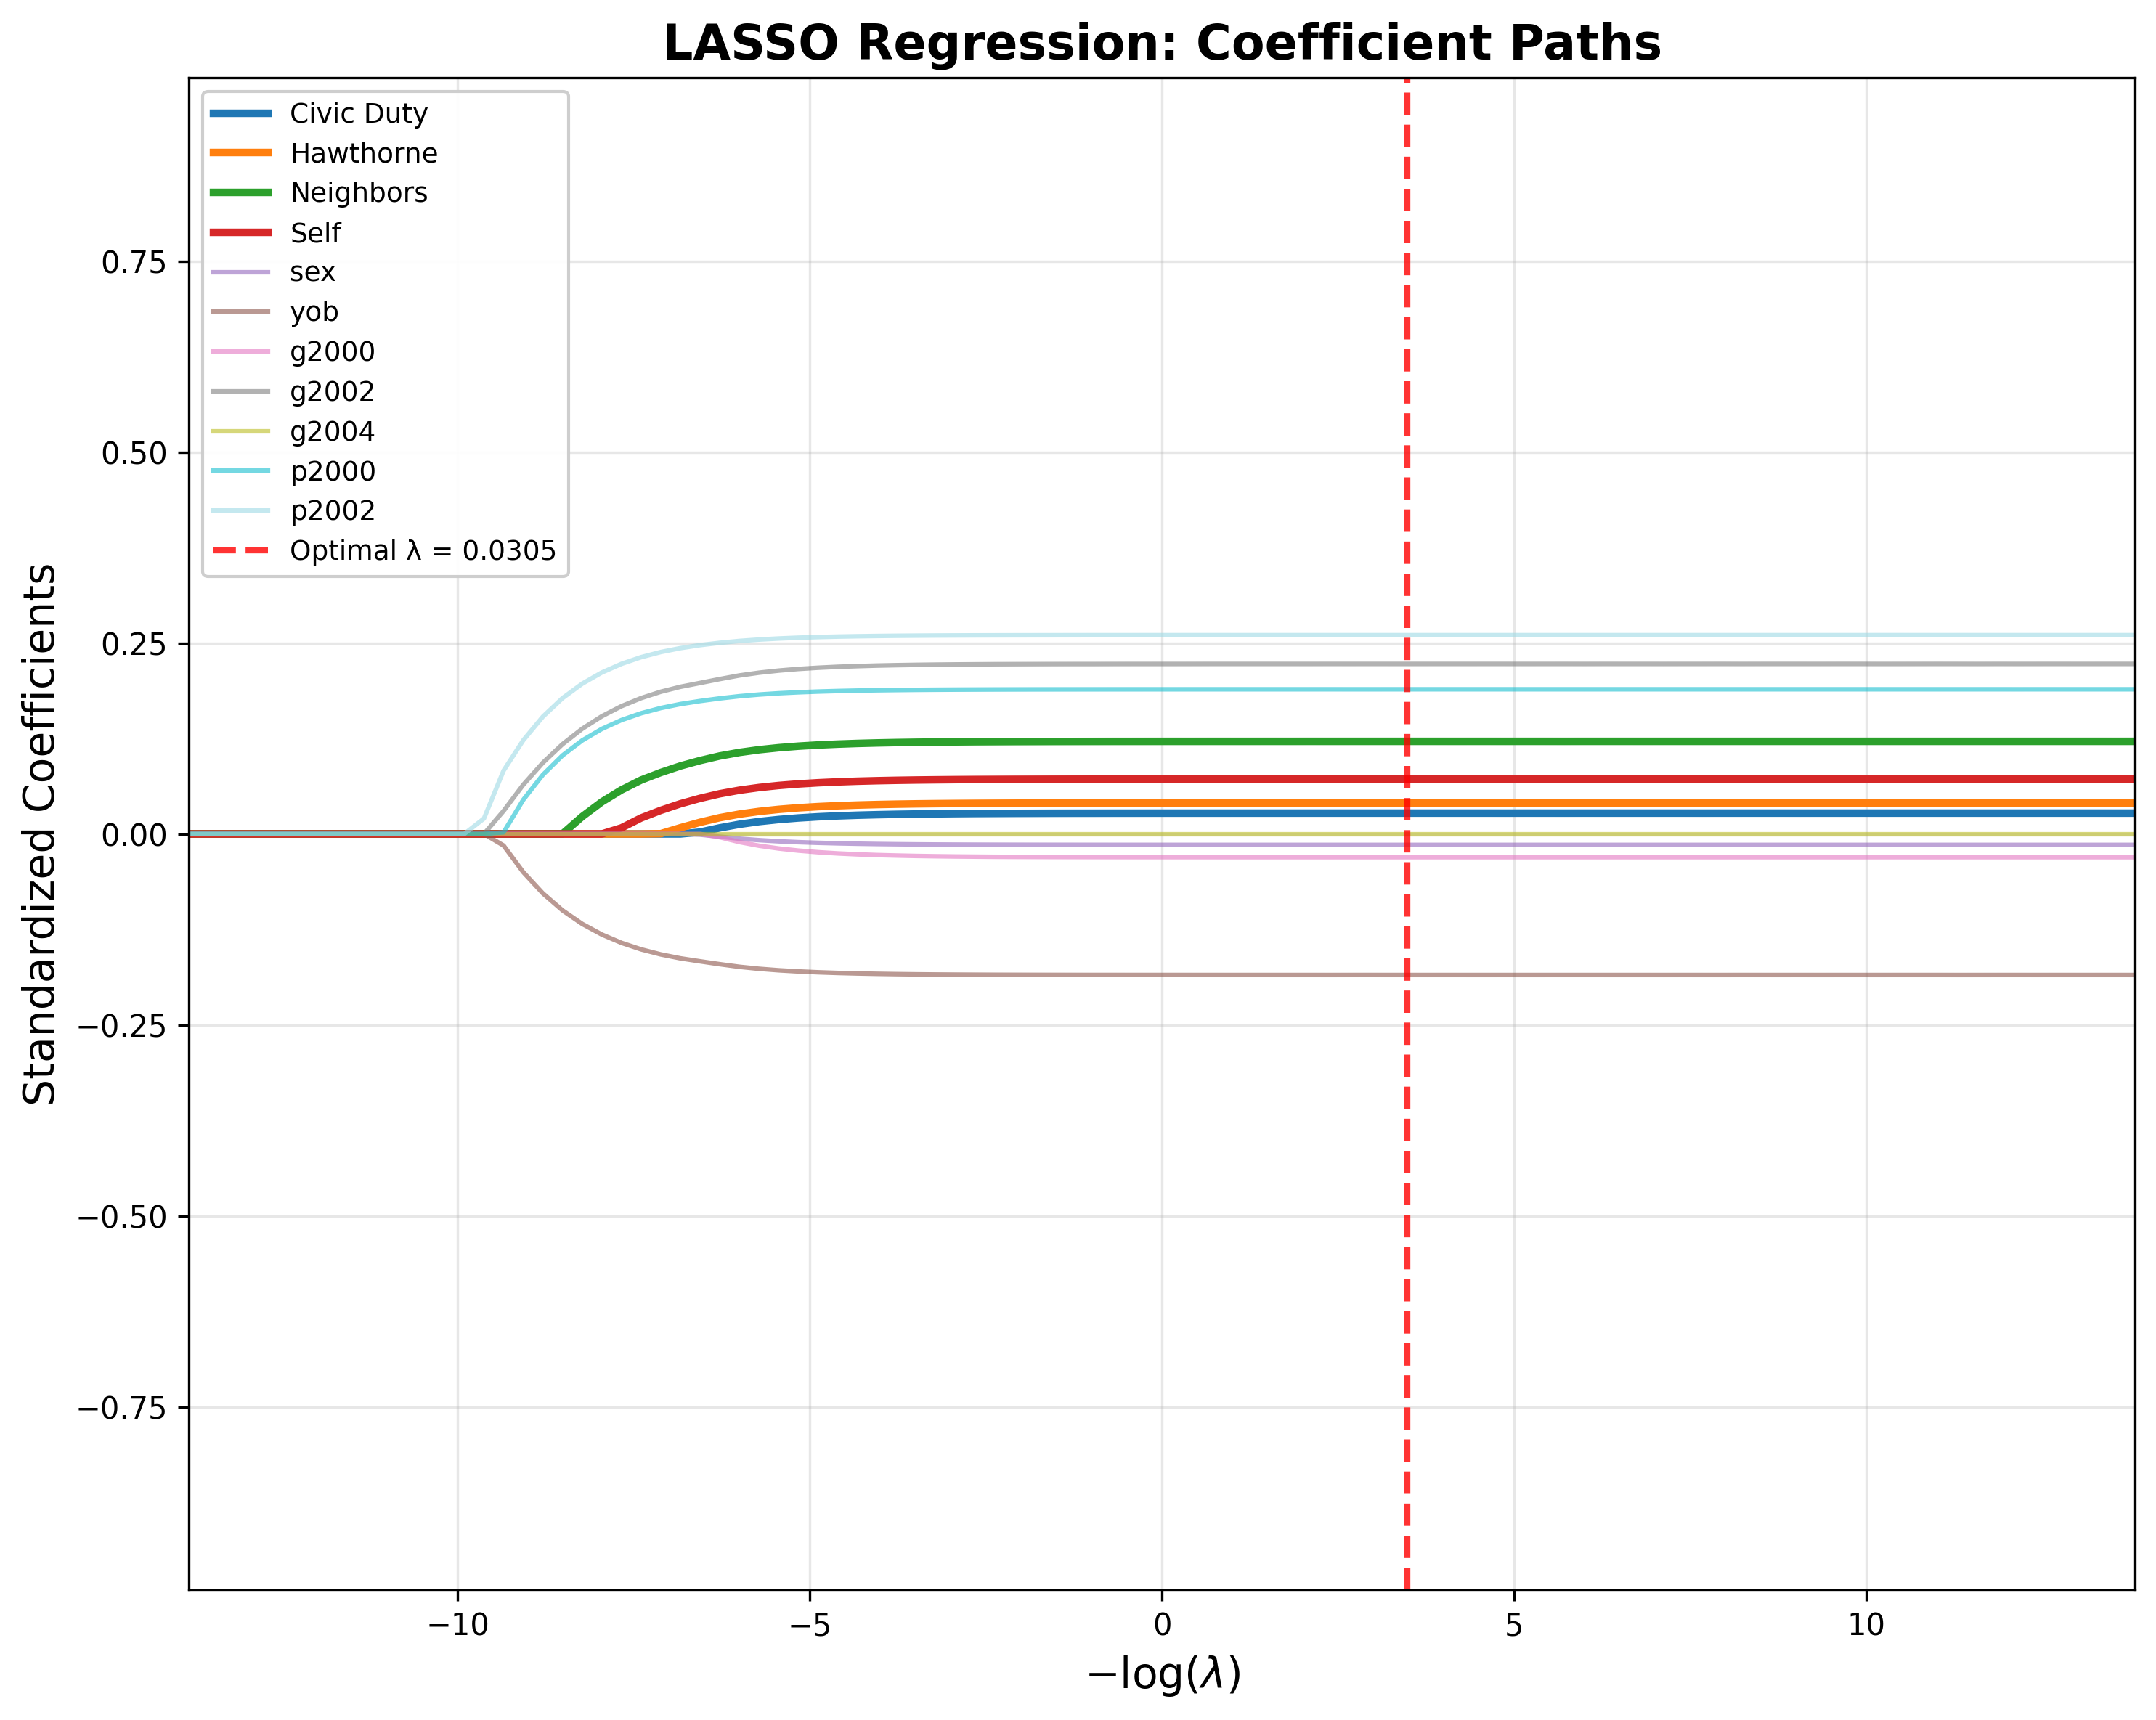
\includegraphics[width=\linewidth]{../Output/Plots/lasso_coefficients.png}
        \vspace{0.3em}
        {\small LASSO coefficient path}
    \end{minipage}
    \hfill
    \begin{minipage}[t]{0.48\textwidth}
        \centering
        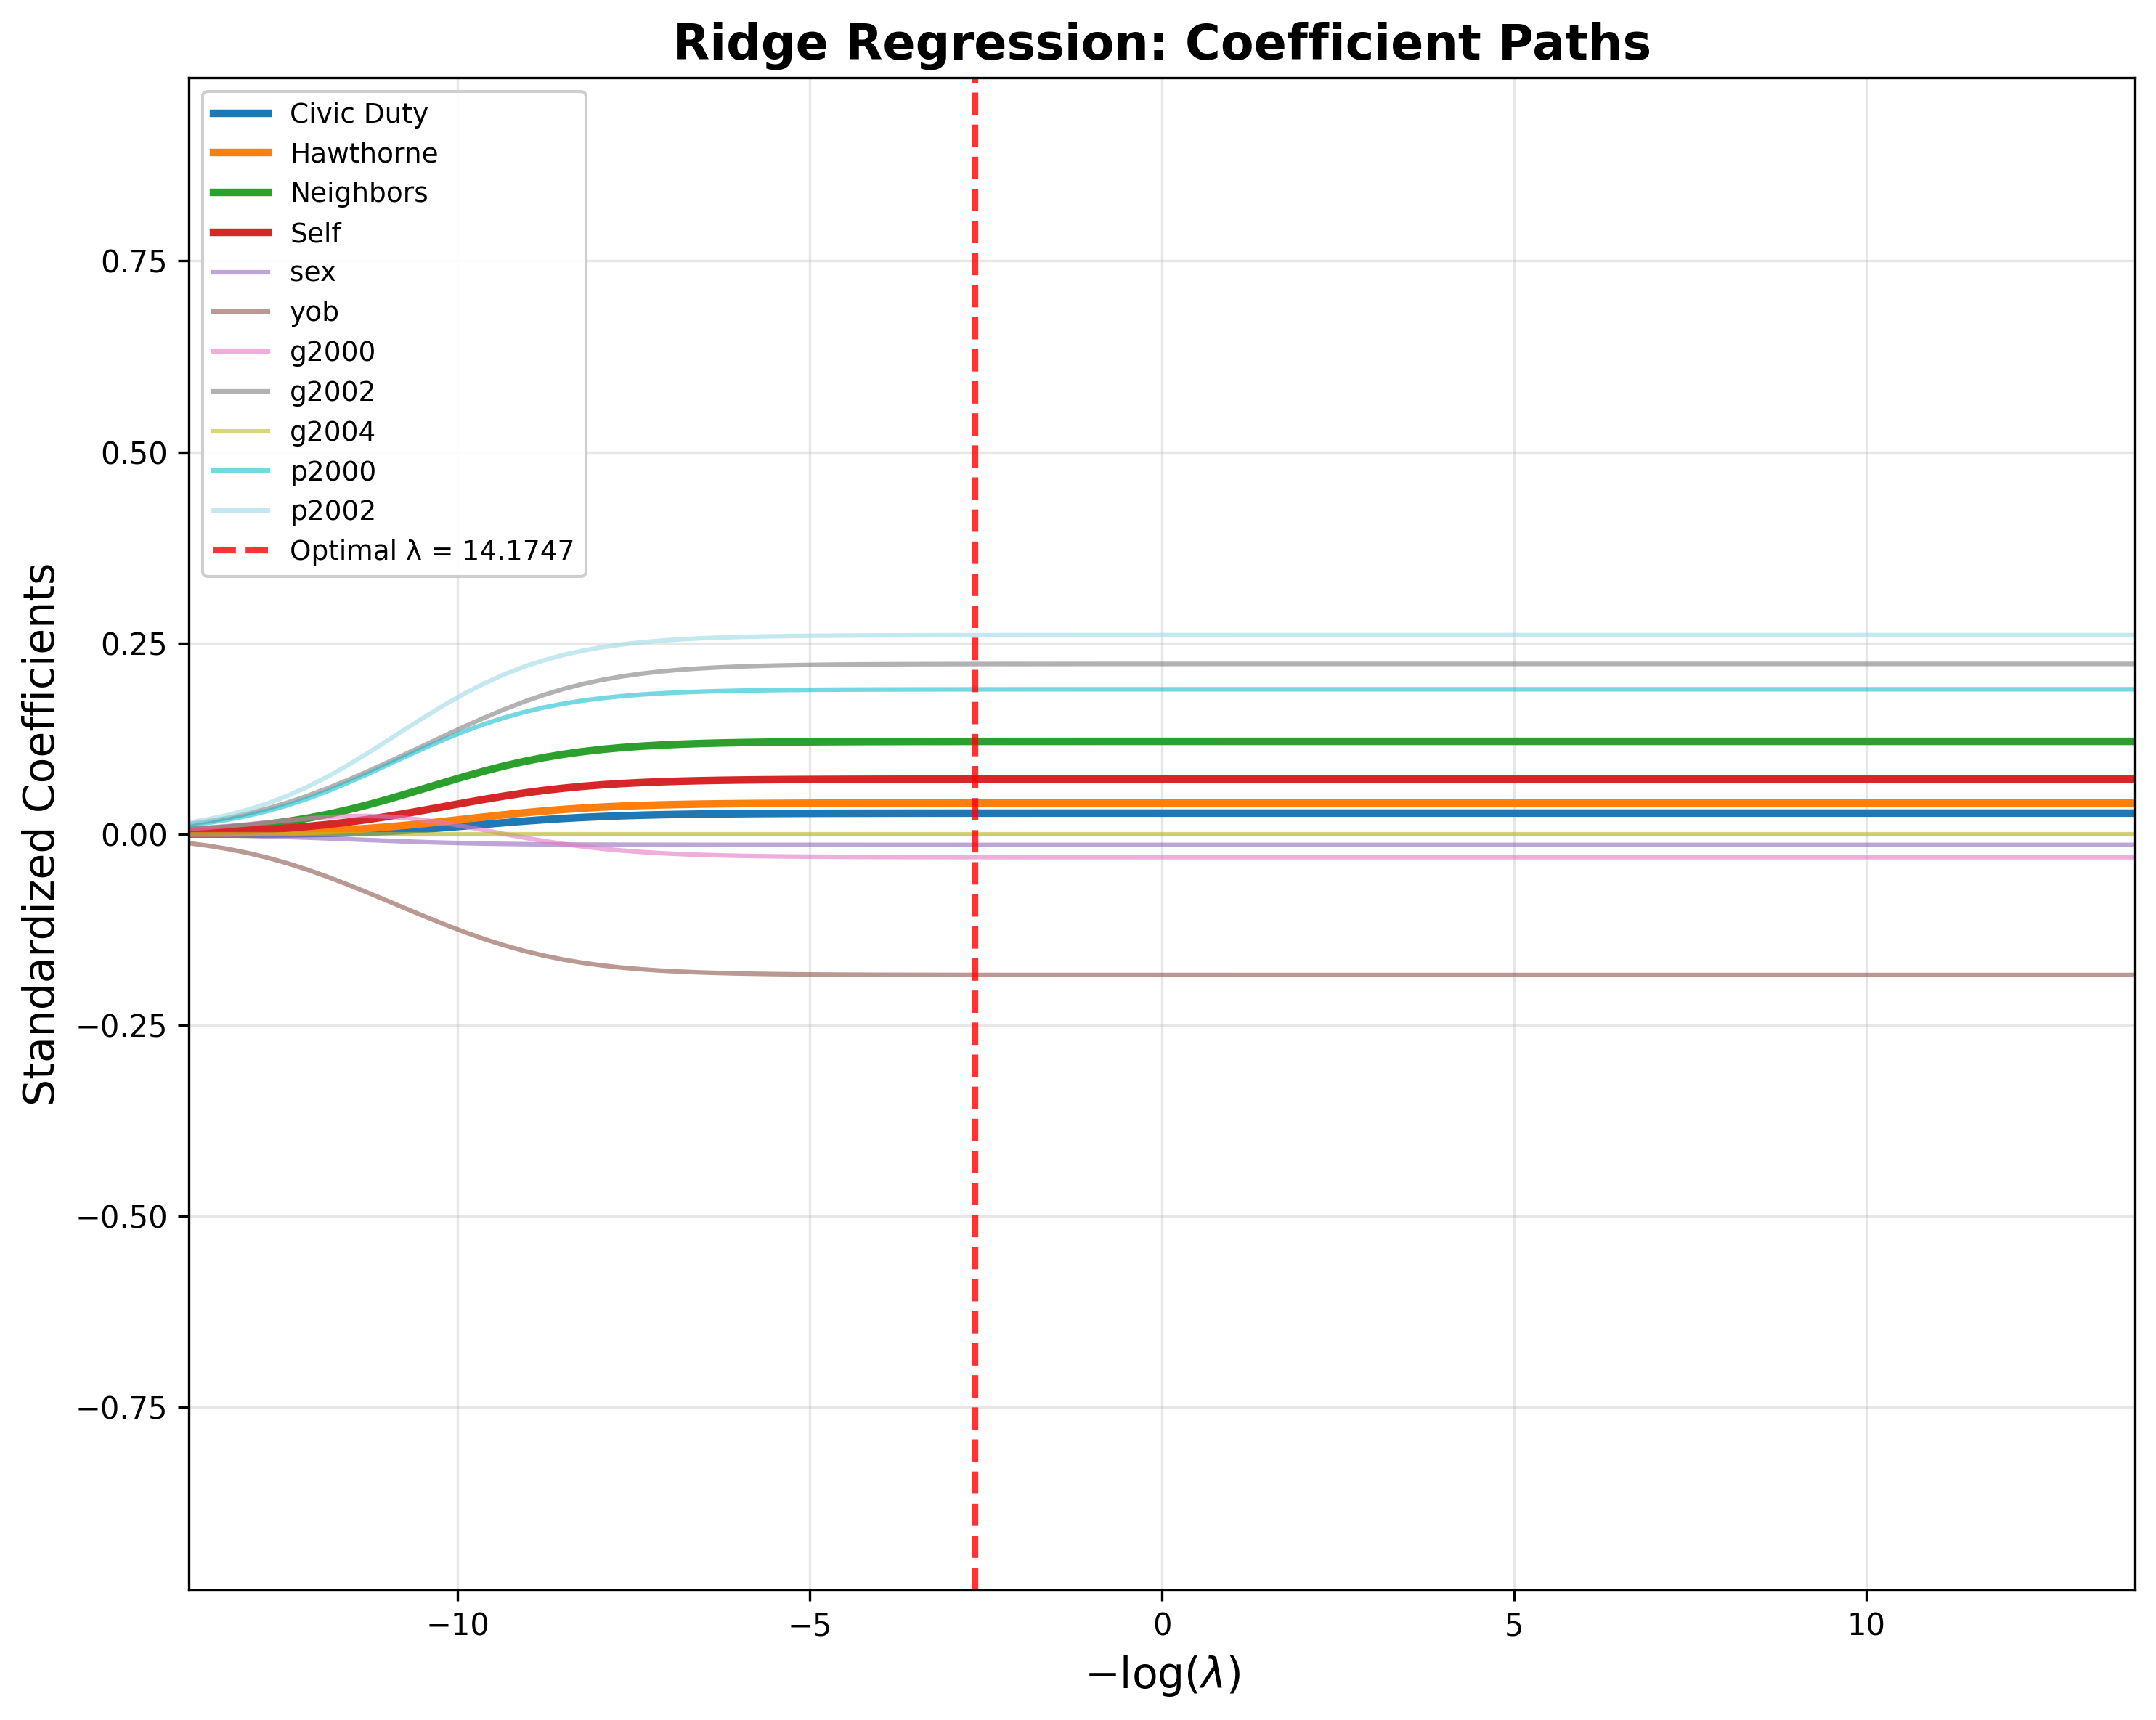
\includegraphics[width=\linewidth]{../Output/Plots/ridge_coefficients.png}
        \vspace{0.3em}
        {\small Ridge coefficient path}
    \end{minipage}
    \caption{Regularization coefficient paths: LASSO (left) and Ridge (right)}
    \label{fig:coef_paths}
\end{figure}

Both the LASSO and Ridge regression coefficient paths show similar patterns with the intensity variables. Ridge showed negative effects for both intensity and high cluster intensity whereas LASSO showed a negative effect for intensity but a positive effect for high cluster intensity. This might be due to the L2 penalty spreading the penalty across all variables unlike the L1 penalty which drives some coefficients to zero.

\subsection{Machine Learning Methods}
To further explore the treatment effects and the potential spillover effects, we will use causal machine learning methods such as Regression Trees, Random Forests, Bagging and Boosting. The results from the random tree are presented below:
\begin{figure}[H]
    \centering
    \includegraphics[width=1\textwidth]{../Output/Plots/diffusion_classification_tree.png}   
    \caption{Regression Tree}
    \label{fig:regression_tree}
\end{figure}
The regression tree shows that the age, previous voting history and the Neighbors treatment are the most important variables in prediction. The regression tree also does not show that cluster intensity is an important variable to be a leading predictor for the outcome variable.

However, the random forest results show that the cluster intensity is an important variable. The variable importance plot is presented below:
\begin{figure}[H]
    \centering
    \includegraphics[width=1\textwidth]{../Output/Plots/random_forest_feature_importance.png}   
    \caption{Random Forest Variable Importance Plot}
    \label{fig:random_forest}
\end{figure}
The random forest importance matrix supports the findings from the regression tree. Age and previous voting history are important predictors, however, neighbourhood demographics and cluster treatment intensity are also important predictors.

Results from the different machine learning models are presented below:
\begin{table}[H]
\caption{Model Comparison: Tree, Forest, Bagging, Boosting}
\label{tab:diffusion_ml_comparison}
\begin{center}
\begin{tabular}{lrrrrrrr}
\toprule
Model & Accuracy & Precision & Recall & F1 & ROC AUC & Log Loss & MSE \\
\midrule
Tree & 0.649 & 0.437 & 0.385 & 0.409 & 0.607 & 6.159 & 0.282 \\
Forest & 0.703 & 0.559 & 0.277 & 0.370 & 0.693 & 0.574 & 0.195 \\
Bagging & 0.615 & 0.429 & 0.660 & 0.520 & 0.679 & 0.640 & 0.225 \\
Boosting & 0.695 & 0.588 & 0.117 & 0.195 & 0.670 & 0.584 & 0.200 \\
\bottomrule
\end{tabular}
\end{center}
\end{table}


It is clear from the results that the Random Forest model performs the best across all metrics. However, boosting provides results that are very close to the Random Forest model. The Random Forest model benefits from the restriction of the predictors to a random subset which highlights that there are strong predictors in the dataset such as age, previous voting history, neighbourhood demographics and cluster treatment intensity.

\subsection{Directed Acyclic Graphs}
Here's a DAG to illustrate the relationships between the variables in our study:
\begin{figure}[H]
    \centering
    \includegraphics[width=0.7\textwidth]{../Output/Plots/dag_plot_3.png}
    \caption{Directed Acyclic Graph (DAG)}
    \label{fig:dag}
\end{figure}
In this DAG, the treatment groups (Civic Duty, Hawthorne, Self, Neighbors) directly influence the outcome variable (Voted in 2006). The control variables as well geographic proximity. (clustering) affects the information sharing node which affects the outcome variable for the control group. Simpler DAGs can be found in the appanedix.

\section{Conclusion}
The results from our statistical analysis clearly show that social pressure treatments have a positive and significant effect on voter turnout. They also show that the control group is influenced by the treatment intensity in their neighbourhood, suggesting that information diffusion effects are present. However, the spillover effects from the Neighbors treatment are not statistically significant in the OLS regression. However, causal machine learning methods suggest that neighbourhood demographics and cluster treatment intensity are important predictors of voter turnout.

This result has important implications for policymakers and businesses. Policymakers can use social pressure treatments to increase voter turnouts and positive diffusion effects allow for more effective mobilization. Businesses can use social pressure treatments along similar lines to increase product adoption and positive word of mouth. 

Spatial clustering in the SAR model also suggest that neighborhood effects matter economically. Business locations and community investments are, thus, spatially dependent decisions that can benefit from understanding the dynamics of information diffusion. There are also business implications to the real estate sector, more civically engaged neighborhoods can lead to more prosperity and economically vibrant communities.

\section{Future Steps}
The next steps are to enhance the robustness of the spatial results with additional tests and to explore the causal machine learning methods that can isolate the spatial diffusion effects more effectively. Once the results are more robust, we can offer more concrete recommendations to policymakers and businesses on how to effectively leverage social pressure and information diffusion to achieve their goals.

Additional extensions can include exploring social media data (such as. X (formerly Twitter)) to see how information diffusion effects spread in the modern age where spatial proximity is less relevant.
\bibliography{references}
\bibliographystyle{chicago}
\end{document}